\documentclass{article}
\documentclass[border=1cm]{standalone}
\usepackage{tikz} 
\usepackage{framed}


\colorlet{tapeBg}{red!30}
\colorlet{tapeBorder}{red!60}

\tikzset{
nodestyle/.style={circle, minimum size=0pt, inner sep=0pt},
boxstyle/.style={rectangle, inner sep = 2pt, outer sep = 0pt, draw, fill=white}
}

% fresh posx posy len
\newcommand{\id}[4]{
  \draw (#2,#3) -- (#2 + #4,#3);
}

% fresh posx posy scaley
\newcommand{\swap}[4]{
 \node [nodestyle] (swapa#1) at (#2,#3) {};
 \node [nodestyle] (swapb#1) at (#2,#3 + #4) {};
 \node [nodestyle] (swapc#1) at (#2+1,#3) {};
 \node [nodestyle] (swapd#1) at (#2+1,#3 + #4) {};
  
 \draw [in=180, out=0] (swapa#1) to (swapd#1);
 \draw [in=-180, out=0] (swapb#1) to (swapc#1);
}

% fresh posx posy otimesdist
\newcommand{\copycirc}[4]{
  \pgfmathsetmacro\pa{#3 + #4 / 2};
  \node [nodestyle] (cpz#1) at (#2,\pa) {};
  \node [circle, minimum size=3pt, fill=black] (cpa#1) at (#2+.5,\pa) {};
  \node [nodestyle] (cpb#1) at (#2+1,#3) {};
  \node [nodestyle] (cpc#1) at (#2+1,#3+#4) {};
  
  \draw (cpz#1) to (cpa#1);
  \draw (cpa#1) to [out=270, in=180] (cpb#1);
  \draw (cpa#1) to [out=90, in=180] (cpc#1);
}

% fresh posx posy
\newcommand{\discardcirc}[3]{
  \node [nodestyle] (cpa#1) at (#2,#3) {};
  \node [circle, minimum size=3pt, fill=black] (cpb#1) at (#2+1,#3) {};
  \draw (cpa#1) to (cpb#1);
}

% fresh posx posy otimesdist
\newcommand{\cocopycirc}[4]{
  \pgfmathsetmacro\pa{#3 + #4 / 2};
  \node [nodestyle] (cpz#1) at (#2+1,\pa) {};
  \node [circle, minimum size=3pt, fill=black] (cpa#1) at (#2+.5,\pa) {};
  \node [nodestyle] (cpb#1) at (#2,#3) {};
  \node [nodestyle] (cpc#1) at (#2,#3+#4) {};
  
  \draw (cpz#1) to (cpa#1);
  \draw (cpa#1) to [out=270, in=0] (cpb#1);
  \draw (cpa#1) to [out=90, in=0] (cpc#1);
}

% fresh posx posy
\newcommand{\codiscardcirc}[3]{
  \node [nodestyle] (cpa#1) at (#2+1,#3) {};
  \node [circle, minimum size=3pt, fill=black] (cpb#1) at (#2,#3) {};
  \draw (cpb#1) to (cpa#1);
}

% fresh posx posy arity coarity name otimesdist
\newcommand{\gen}[7]{
  \node [color=gray] () at (#2, #3) {$\bot$};
  \pgfmathsetmacro\arity{#4};
  \pgfmathsetmacro\coarity{#5};
  \pgfmathsetmacro\otimesdist{#7};

\pgfmathparse{%
  \arity - 1
}%
\let\arminone\pgfmathresult

\pgfmathparse{%
  \coarity - 1
}%
\let\coarminone\pgfmathresult

\pgfmathparse{%
  (\arity>\coarity)
    ? \arminone * \otimesdist
    : \coarminone * \otimesdist
}%
\let\height\pgfmathresult

\pgfmathparse{%
  \arminone * \otimesdist * 0.5
}%
\let\leftboxheight\pgfmathresult

\pgfmathparse{%
  \coarminone * \otimesdist * 0.5
}%
\let\rightboxheight\pgfmathresult

% this node is the bottom of the left interface of the box
\node [] (a) at (#2 + 1,#3 + \height / 2 - \leftboxheight / 2) {};
% this node is the bottom of the right interface of the box
\node [] (b) at (#2 + 1,#3 + \height / 2 - \rightboxheight / 2) {};

\pgfmathparse{%
  (\arity - 1) / 2 * \otimesdist
}%
\let\arshift\pgfmathresult

%draw left connections
\pgfmathparse{%
  (\coarity - 1) / 2 * \otimesdist
  }%
\let\coarshift\pgfmathresult

  \ifnum \arity=0\else
   \foreach \i in {0,...,\arminone}
  {
    \node [nodestyle] (#1in\i) at (#2, #3 + \i * \otimesdist + \height / 2 - \arshift) {};

    \draw[in=0, out=180] (a) ++ (0,\i * \otimesdist * 0.5) to (#1in\i);
  }
  
  \fi

  %draw right connections
  \ifnum \coarity=0\else
  \foreach \i in {0,...,\coarminone}
  {
    \node [nodestyle] (#1out\i) at (#2 + 2, #3 + \i * \otimesdist + \height / 2 - \coarshift) {};

    \draw[in=180, out=0] (b) ++ (0,\i * \otimesdist * 0.5) to (#1out\i);
  }
  \fi
  
  \pgfmathsetmacro\boxheight{\height / 2 + \otimesdist}
  
  %draw box with name
  \node [boxstyle, minimum height = \boxheight cm] at (#2 + 1,#3 + \height / 2) {#6};
}


% posx posy width height
\newcommand{\tape}[4]{
  \draw [fill=tapeBg, tapeBg] (#1, #2) -- (#1+#3, #2) -- (#1+#3, #2+#4) -- (#1, #2+#4) -- cycle;
  
  \draw[tapeBorder, line width=0.5pt] (#1, #2) -- (#1+#3, #2);
  \draw[tapeBorder, line width=0.5pt] (#1+#3, #2+#4) -- (#1, #2+#4);
}

% posxll posyll posxlu posylu posxrl posyrl posxru posyru
\newcommand{\freestyletape}[8]{
  \draw [fill=tapeBg, tapeBg] (#1, #2) -- (#3, #4) [in=180, out=0] to (#7, #8) -- (#5, #6)  [in=0, out=180] to cycle;

   \draw[tapeBorder, line width=0.5pt, in=180, out=0] (#1, #2) to (#5, #6);
  \draw[tapeBorder, line width=0.5pt, in=180, out=0] (#3, #4) to (#7, #8);
}

% posx posy h1 h2 
\newcommand{\adapter}[4] {
  \draw [fill=tapeBg, tapeBg] (#1, #2 - #3 / 2) -- (#1, #2 + #3 / 2) -- (#1+0.5, #2+#4/2) -- (#1+0.5, #2 - #4 / 2) -- cycle;
}


% posx posy n1 n2 oplusdist otimesdist tapepadding width
\newcommand{\swaptape}[8]{
  \pgfmathsetmacro{\posx}{#1}
  \pgfmathsetmacro{\posy}{#2}
  \pgfmathsetmacro{\none}{#3}
  \pgfmathsetmacro{\ntwo}{#4}
  \pgfmathsetmacro{\oplusdist}{#5}
  \pgfmathsetmacro{\otimesdist}{#6}
  \pgfmathsetmacro{\tapepadding}{#7}
  \pgfmathsetmacro{\width}{#8}

   \ifnum\none=0
      \pgfmathsetmacro{\sizeone}{2 * \tapepadding}
    \else
      \pgfmathsetmacro{\sizeone}{(\none - 1) * \otimesdist + (2 * \tapepadding)}
    \fi

    \ifnum\ntwo=0
      \pgfmathsetmacro{\sizetwo}{2 * \tapepadding}
    \else
      \pgfmathsetmacro{\sizetwo}{(\ntwo - 1) * \otimesdist + (2 * \tapepadding)}
    \fi

    \pgfmathsetmacro{\twobasebotx}{\posx}
    \pgfmathsetmacro{\twobaseboty}{\posy}

    \pgfmathsetmacro{\twoceilbotx}{\posx}
    \pgfmathsetmacro{\twoceilboty}{\posy + \sizetwo}

    \pgfmathsetmacro{\twobasetopx}{\posx + \width}
    \pgfmathsetmacro{\twobasetopy}{\posy + \sizeone + \oplusdist}

    \pgfmathsetmacro{\twoceiltopx}{\posx + \width}
    \pgfmathsetmacro{\twoceiltopy}{\posy + \sizeone + \oplusdist + \sizetwo}

    \pgfmathsetmacro{\onebasebotx}{\posx + \width}
    \pgfmathsetmacro{\onebaseboty}{\posy}

    \pgfmathsetmacro{\oneceilbotx}{\posx + \width}
    \pgfmathsetmacro{\oneceilboty}{\posy + \sizeone}

    \pgfmathsetmacro{\onebasetopx}{\posx}
    \pgfmathsetmacro{\onebasetopy}{\posy + \sizetwo + \oplusdist}

    \pgfmathsetmacro{\oneceiltopx}{\posx}
    \pgfmathsetmacro{\oneceiltopy}{\posy + \sizetwo + \oplusdist + \sizeone}

    \draw [fill=tapeBg, tapeBg, in=180, out=0] (\twobasebotx, \twobaseboty) to (\twobasetopx, \twobasetopy) --  (\twoceiltopx, \twoceiltopy) [in=0, out=180] to (\twoceilbotx, \twoceilboty) -- cycle;

    \draw [fill=tapeBg, tapeBg, in=0, out=180] (\onebasebotx, \onebaseboty) to (\onebasetopx, \onebasetopy) --  (\oneceiltopx, \oneceiltopy) [in=180, out=0] to (\oneceilbotx, \oneceilboty) -- cycle;

    \draw[tapeBorder, in=180, out=0] (\twobasebotx, \twobaseboty) to (\twobasetopx, \twobasetopy);
    \draw[tapeBorder, in=180, out=0] (\twoceilbotx, \twoceilboty) to (\twoceiltopx, \twoceiltopy);


    \draw[tapeBorder, in=0, out=180] (\onebasebotx, \onebaseboty) to (\onebasetopx, \onebasetopy);
    \draw[tapeBorder, in=0, out=180] (\oneceilbotx, \oneceilboty) to (\oneceiltopx, \oneceiltopy);


    \foreach \i in {0,...,\ntwo}
    {
      \pgfmathsetmacro{\iminone}{\i - 1}
      \ifnum\i=0
    \else
      \draw[in=180, out=0] (\twobasebotx, \twobaseboty + \iminone * \otimesdist + \tapepadding) to (\twobasetopx, \twobasetopy + \iminone * \otimesdist + \tapepadding);
    \fi
    }

    \foreach \i in {0,...,\none}
    {
    \pgfmathsetmacro{\iminone}{\i - 1}
     \ifnum\i=0
    \else
      \draw[in=0, out=180] (\oneceilbotx, \onebaseboty + \iminone * \otimesdist + \tapepadding) to   (\onebasetopx, \onebasetopy + (\iminone * \otimesdist + \tapepadding);
    \fi



    }


}


% posx, posy, n, lminone, paddingdist, otimesdist, oplusdist
\newcommand{\splittape}[7] {
  \pgfmathsetmacro{\posx}{#1}
  \pgfmathsetmacro{\posy}{#2}
  \pgfmathsetmacro{\n}{#3}
  \pgfmathsetmacro{\l}{#4}
  \pgfmathsetmacro{\paddingdist}{#5}
  \pgfmathsetmacro{\otimesdist}{#6}
  \pgfmathsetmacro{\oplusdist}{#7}
  
  \pgfmathparse{%
    (\n>0)
      ? 2 * \paddingdist + (\n - 1) * \otimesdist
      : 2 * \paddingdist
  }%
  \let\h\pgfmathresult
  
  \pgfmathsetmacro{\diff}{(\oplusdist - \h) / 2}
  
   \draw [fill=tapeBg, tapeBg] (\posx, \posy + \h + \diff) -- (\posx + 1, \posy + \h + \diff) [out = 270, in = 180] to (\posx +1 + \l, \posy) [in = 270, out = 90] to (\posx +1 + \l, \posy + \h) to [out = 180, in = 270] (\posx + 1 + 2 * \l/3, \posy + \h + \h/2 + \diff) to [out = 90, in = 180] (\posx +1 + \l, \posy + \h + \oplusdist) -- (\posx +1 + \l, \posy + 2*\h + \oplusdist) to [out = 180, in = 90] (\posx + 1, \posy + 2*\h + \diff) -- (\posx, \posy + 2 * \h + \diff) -- cycle;
  
  \draw[tapeBorder, line width=0.5pt] (\posx, \posy + \h + \diff) -- (\posx + 1, \posy + \h + \diff) [out = 270, in = 180] to (\posx +1 + \l, \posy);
  
  \draw[tapeBorder, line width=0.5pt] (\posx, \posy + 2*\h + \diff) -- (\posx + 1, \posy + 2*\h + \diff) [out = 90, in = 180] to (\posx +1 + \l, \posy + 2*\h + \oplusdist);
  
  \draw [tapeBorder, line width=0.5pt] (\posx +1 + \l, \posy + \h + \oplusdist) [in = 90, out= 180] to (\posx + 1 +  2 * \l/3, \posy + \h + \h/2 + \diff) [in = 180, out= 270] to (\posx +1 + \l, \posy + \h);
  
  
   \foreach \i in {0,...,\n}
    {
      \ifnum\i=0
    \else
     \pgfmathsetmacro{\ishift}{(\i - 1) * \otimesdist}
      
       \draw[line width=0.5pt] (\posx, \posy + \h + \diff + \paddingdist + \ishift) -- 
      (\posx + 1 + \paddingdist, \posy + \h + \diff + \paddingdist + \ishift) [out = 270, in = 180] to (\posx +1 + \l, \posy + \paddingdist + \ishift);
      \draw[line width=0.5pt] (\posx, \posy + \h + \diff + \paddingdist + \ishift) -- 
      (\posx + 1 + \paddingdist, \posy + \h + \diff + \paddingdist + \ishift) [out = 90, in = 180] to (\posx +1 + \l, \posy + \h + \oplusdist + \paddingdist + \ishift);
    \fi
    }
  
}

% posx, posy, n, paddingdist, otimesdist
\newcommand{\cuttape}[5]{
  \pgfmathsetmacro{\posx}{#1}
  \pgfmathsetmacro{\posy}{#2}
  \pgfmathsetmacro{\n}{#3}
  \pgfmathsetmacro{\paddingdist}{#4}
  \pgfmathsetmacro{\otimesdist}{#5}
  \pgfmathparse{%
    (\n>0)
      ? 2 * \paddingdist + (\n - 1) * \otimesdist
      : 2 * \paddingdist
  }%
  \let\h\pgfmathresult
    \pgfmathsetmacro{\otimesdist}{#5}
    \pgfmathparse{%
    (\n>0)
      ? \n * \otimesdist
      : 1
  }%
  \let\l\pgfmathresult
  
  
  \draw [tapeBg, fill = tapeBg] (\posx, \posy) -- (\posx, \posy + \h) -- (\posx + \l / 2, \posy + \h)  [out = 0, in = 90] to (\posx + \l, \posy + \h/2) [out = 270, in = 0] to (\posx + \l / 2, \posy) -- cycle;
  
     \foreach \i in {0,...,\n}
    {
      \ifnum\i=0
    \else
     \pgfmathsetmacro{\ishift}{\paddingdist + (\i - 1) * \otimesdist}
      \draw (\posx, \posy + \ishift) -- (\posx + \l, \posy + \ishift);
    \fi
    }
  
  \draw [white, fill=white] (\posx + \l / 2, \posy + \h)  [out = 0, in = 90] to (\posx + \l, \posy + \h/2) [out = 270, in = 0] to (\posx + \l / 2, \posy) -- (\posx + \l + 0.2, \posy) -- (\posx + \l + 0.2, \posy + \h) -- cycle;
  
  \draw [tapeBorder] (\posx, \posy + \h) -- (\posx + \l / 2, \posy + \h)  [out = 0, in = 90] to (\posx + \l, \posy + \h/2) [out = 270, in = 0] to (\posx + \l / 2, \posy) -- (\posx, \posy);
}

% posx, posy, n, lminone, paddingdist, otimesdist, oplusdist
\newcommand{\jointape}[7] {
  \pgfmathsetmacro{\posx}{#1}
  \pgfmathsetmacro{\posy}{#2}
  \pgfmathsetmacro{\n}{#3}
  \pgfmathsetmacro{\l}{#4}
  \pgfmathsetmacro{\paddingdist}{#5}
  \pgfmathsetmacro{\otimesdist}{#6}
  \pgfmathsetmacro{\oplusdist}{#7}
  
  \pgfmathparse{%
    (\n>0)
      ? 2 * \paddingdist + (\n - 1) * \otimesdist
      : 2 * \paddingdist
  }%
  \let\h\pgfmathresult
  
  \pgfmathsetmacro{\centerposx}{\posx + (\l + 1) / 2}
  \pgfmathsetmacro{\centerposy}{\posy + (2 * \h + \oplusdist)/2}
  
  \node() at (\centerposx, \centerposy) {
    \reflectbox{\begin{tikzpicture}
     \splittape{#1}{#2}{#3}{#4}{#5}{#6}{#7}
    \end{tikzpicture}}

  };
}

% posx, posy, n, paddingdist, otimesdist
\newcommand{\spawntape}[5] {
  \pgfmathsetmacro{\posx}{#1}
  \pgfmathsetmacro{\posy}{#2}
  \pgfmathsetmacro{\n}{#3}
  \pgfmathsetmacro{\paddingdist}{#4}
  \pgfmathsetmacro{\otimesdist}{#5}
    \pgfmathparse{%
    (\n>0)
      ? 2 * \paddingdist + (\n - 1) * \otimesdist
      : 2 * \paddingdist
  }%
  \let\h\pgfmathresult
  
  \pgfmathsetmacro{\otimesdist}{#5}
    \pgfmathparse{%
    (\n>0)
      ? \n * \otimesdist - 0.2
      : 1 - 0.2
  }%
  \let\l\pgfmathresult
  
  \pgfmathsetmacro{\centerposx}{\posx + (\l) / 2}
  \pgfmathsetmacro{\centerposy}{\posy + (\h) /2}
  
  \node() at (\centerposx, \centerposy) {
    \reflectbox{\begin{tikzpicture}
     \cuttape{#1}{#2}{#3}{#4}{#5}
    \end{tikzpicture}}

  };
}

% fresh name, len, posx, posy
\newcommand{\measuretape}[4]{
  \pgfmathsetmacro{\len}{#2 * 1}

  \node [nodestyle] (measa#1) at (#3,#4) {};
  \node [nodestyle] (measb#1) at (#3,#4+#2) {};
  \node [nodestyle] () at (#3,#4+#2+.3) {$\len$};
  \draw [|-|] (measa#1) -- (measb#1);
}



 


\begin{document}

\subsection{The Language}

A program in the language we provide consists of a series of declarations and commands. The former are used to define sorts, terms of a sesquistrict rig signature and tape diagrams, whereas the latter can be used to act on them, e.g. to typecheck, draw, or otherwise manipulate the terms and diagrams. The following is the BNF representation of a program $p$:
\begin{align*}
 p &::= com \mid d \mid p \texttt{.} p\\
 d &::= \texttt{let}\; v \texttt{:}\,type\;\texttt{=}\; e \mid \texttt{let}\; v : \texttt{sort}\\
 com &::= \texttt{check} \;e \mid \texttt{draw} \;e \text{ to } path \mid \text{\color{red} Add other commands here}\\
 e &::= v \mid SSR \mid TD\\
 type &::= \texttt{tape} \mid \texttt{term}
\end{align*}
Where $v$ is a variable name, $SSR$ is a term of a sesquistrict rig signature and $TD$ is a tape diagram. In the language:

\begin{itemize}
 \item The $\otimes$ and $\oplus$ symbols are notated as \texttt{*} and \texttt{+}.
 \item The symmetries $\sigma^{\otimes}_{\bullet, \bullet}$ and $\sigma^{\oplus}_{\bullet, \bullet}$ are notated as \texttt{s*($\bullet, \bullet$)} and \texttt{s+($\bullet, \bullet$)}.
 \item The left distributor $\delta^l_{\bullet, \bullet, \bullet}$ is notated as \texttt{dl($\bullet, \bullet, \bullet$)}.
 \item The named generators are written as:
\[ \tt gen(name, arity, coarity) \]
 \item A circuit enclosed in a tape, i.e. $\underline{\overline{c}}$, is notated as \texttt{[c]}
\end{itemize}
As an example, the following is a valid program:
\begin{lstlisting}[language = , label = lst:example, caption=Example program]
let A : sort.   let B : sort.   let C : sort.
let t : tape = id(A + B) ; s+(A, B).

check t.                          // true
check id(A) ; id(B).              // false
draw t to "./figure1.txt".
draw s*(A + B, C) to "./figure2.txt"
\end{lstlisting}

\begin{figure}[ht]
\ctbox{
 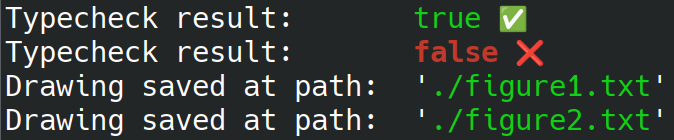
\includegraphics[scale = .4]{imgs/result}
 }
 \caption{Result of the program in Listing \ref{lst:example}.}
\end{figure}

\begin{figure}[ht]
\ctbox{
\begin{tikzpicture}
 \freestyletape {4.000000} {1.500000} {4.000000} {2.500000} {5.000000} {1.500000} {5.000000} {2.500000}\draw [in=180, out=0] (4.000000 , 2.000000) to (5.000000 , 2.000000);
\freestyletape {4.000000} {0.000000} {4.000000} {1.000000} {5.000000} {0.000000} {5.000000} {1.000000}\draw [in=180, out=0] (4.000000 , 0.500000) to (5.000000 , 0.500000);
\freestyletape {1.000000} {1.500000} {1.000000} {2.500000} {2.000000} {1.500000} {2.000000} {2.500000}\draw [in=180, out=0] (1.000000 , 2.000000) to (2.000000 , 2.000000);
\freestyletape {1.000000} {0.000000} {1.000000} {1.000000} {2.000000} {0.000000} {2.000000} {1.000000}\draw [in=180, out=0] (1.000000 , 0.500000) to (2.000000 , 0.500000);
\tape {0.000000} {1.500000} {1.000000} {1.000000}
\id{2}{0.000000}{2.000000}
\tape {0.000000} {0.000000} {1.000000} {1.000000}
\id{1}{0.000000}{0.500000}
\freestyletape {1.000000} {1.500000} {1.000000} {2.500000} {1.000000} {1.500000} {1.000000} {2.500000}\draw [in=180, out=0] (1.000000 , 2.000000) to (1.000000 , 2.000000);
\freestyletape {1.000000} {0.000000} {1.000000} {1.000000} {1.000000} {0.000000} {1.000000} {1.000000}\draw [in=180, out=0] (1.000000 , 0.500000) to (1.000000 , 0.500000);
\swaptape {2.000000} {0.000000} {1} {1} {0.500000} {1.000000} {0.500000} {2.000000}\tape {5.000000} {1.500000} {1.000000} {1.000000}
\id{4}{5.000000}{2.000000}
\tape {5.000000} {0.000000} {1.000000} {1.000000}
\id{3}{5.000000}{0.500000}
\freestyletape {6.000000} {1.500000} {6.000000} {2.500000} {6.000000} {1.500000} {6.000000} {2.500000}\draw [in=180, out=0] (6.000000 , 2.000000) to (6.000000 , 2.000000);
\freestyletape {6.000000} {0.000000} {6.000000} {1.000000} {6.000000} {0.000000} {6.000000} {1.000000}\draw [in=180, out=0] (6.000000 , 0.500000) to (6.000000 , 0.500000);

\node () at (-0.500000, 2.000000) {A};
\node () at (-0.500000, 0.500000) {B};
\node () at (6.500000, 2.000000) {B};
\node () at (6.500000, 0.500000) {A};
\end{tikzpicture}

 }
 \caption{Image encoded in \text{figure1.txt}, written by the program in Listing \ref{lst:example}.}
\end{figure}


\begin{figure}[ht]
\ctbox{
\begin{tikzpicture}
 \freestyletape {1.000000} {2.500000} {1.000000} {4.500000} {2.000000} {2.500000} {2.000000} {4.500000}\draw [in=180, out=0] (1.000000 , 4.000000) to (2.000000 , 4.000000);
\draw [in=180, out=0] (1.000000 , 3.000000) to (2.000000 , 3.000000);
\freestyletape {1.000000} {0.000000} {1.000000} {2.000000} {2.000000} {0.000000} {2.000000} {2.000000}\draw [in=180, out=0] (1.000000 , 1.500000) to (2.000000 , 1.500000);
\draw [in=180, out=0] (1.000000 , 0.500000) to (2.000000 , 0.500000);
\tape {0.000000} {2.500000} {1.000000} {2.000000}
\id{8}{0.000000}{4.000000}
\id{7}{0.000000}{3.000000}
% adjusting misaligned tensors:
\draw [in=180, out=0] (1.000000 , 4.000000) to (1.000000 , 4.000000);
\draw [in=180, out=0] (1.000000 , 3.000000) to (1.000000 , 3.000000);
\tape {0.000000} {0.000000} {1.000000} {2.000000}
\id{6}{0.000000}{1.500000}
\id{5}{0.000000}{0.500000}
% adjusting misaligned tensors:
\draw [in=180, out=0] (1.000000 , 1.500000) to (1.000000 , 1.500000);
\draw [in=180, out=0] (1.000000 , 0.500000) to (1.000000 , 0.500000);
\freestyletape {1.000000} {2.500000} {1.000000} {4.500000} {1.000000} {2.500000} {1.000000} {4.500000}\draw [in=180, out=0] (1.000000 , 4.000000) to (1.000000 , 4.000000);
\draw [in=180, out=0] (1.000000 , 3.000000) to (1.000000 , 3.000000);
\freestyletape {1.000000} {0.000000} {1.000000} {2.000000} {1.000000} {0.000000} {1.000000} {2.000000}\draw [in=180, out=0] (1.000000 , 1.500000) to (1.000000 , 1.500000);
\draw [in=180, out=0] (1.000000 , 0.500000) to (1.000000 , 0.500000);
\tape {2.000000} {2.500000} {3.000000} {2.000000}
\id{14}{2.000000}{4.000000}
\id{13}{2.000000}{3.000000}
% adjusting misaligned tensors:
\draw [in=180, out=0] (3.000000 , 4.000000) to (3.000000 , 4.000000);
\draw [in=180, out=0] (3.000000 , 3.000000) to (3.000000 , 3.000000);
\swap{2}{3.000000}{3.000000}{1.000000}
% composing interfaces:
\draw [in=180, out=0] (3.000000 , 4.000000) to (3.000000 , 4.000000);
\draw [in=180, out=0] (3.000000 , 3.000000) to (3.000000 , 3.000000);
\id{16}{4.000000}{4.000000}
\id{15}{4.000000}{3.000000}
% adjusting misaligned tensors:
\draw [in=180, out=0] (5.000000 , 4.000000) to (5.000000 , 4.000000);
\draw [in=180, out=0] (5.000000 , 3.000000) to (5.000000 , 3.000000);
% composing interfaces:
\draw [in=180, out=0] (4.000000 , 4.000000) to (4.000000 , 4.000000);
\draw [in=180, out=0] (4.000000 , 3.000000) to (4.000000 , 3.000000);
\tape {2.000000} {0.000000} {3.000000} {2.000000}
\id{10}{2.000000}{1.500000}
\id{9}{2.000000}{0.500000}
% adjusting misaligned tensors:
\draw [in=180, out=0] (3.000000 , 1.500000) to (3.000000 , 1.500000);
\draw [in=180, out=0] (3.000000 , 0.500000) to (3.000000 , 0.500000);
\swap{1}{3.000000}{0.500000}{1.000000}
% composing interfaces:
\draw [in=180, out=0] (3.000000 , 1.500000) to (3.000000 , 1.500000);
\draw [in=180, out=0] (3.000000 , 0.500000) to (3.000000 , 0.500000);
\id{12}{4.000000}{1.500000}
\id{11}{4.000000}{0.500000}
% adjusting misaligned tensors:
\draw [in=180, out=0] (5.000000 , 1.500000) to (5.000000 , 1.500000);
\draw [in=180, out=0] (5.000000 , 0.500000) to (5.000000 , 0.500000);
% composing interfaces:
\draw [in=180, out=0] (4.000000 , 1.500000) to (4.000000 , 1.500000);
\draw [in=180, out=0] (4.000000 , 0.500000) to (4.000000 , 0.500000);
\freestyletape {5.000000} {2.500000} {5.000000} {4.500000} {5.000000} {2.500000} {5.000000} {4.500000}\draw [in=180, out=0] (5.000000 , 4.000000) to (5.000000 , 4.000000);
\draw [in=180, out=0] (5.000000 , 3.000000) to (5.000000 , 3.000000);
\freestyletape {5.000000} {0.000000} {5.000000} {2.000000} {5.000000} {0.000000} {5.000000} {2.000000}\draw [in=180, out=0] (5.000000 , 1.500000) to (5.000000 , 1.500000);
\draw [in=180, out=0] (5.000000 , 0.500000) to (5.000000 , 0.500000);

\node () at (-0.500000, 4.000000) {A};
\node () at (-0.500000, 3.000000) {C};
\node () at (-0.500000, 1.500000) {B};
\node () at (-0.500000, 0.500000) {C};
\node () at (5.500000, 4.000000) {C};
\node () at (5.500000, 3.000000) {A};
\node () at (5.500000, 1.500000) {C};
\node () at (5.500000, 0.500000) {B};




\end{tikzpicture}

 }
 \caption{Image encoded in \text{figure2.txt}, written by the program in Listing \ref{lst:example}.}
\end{figure}


\end{document}
